\chapter{Literature Review} \label{Chp: LiteratureReview}

In this chapter, we will start by introducing the building components of WSN, mainly focuses on different protocol options at each layer. Then we move to security related work, in three aspects of traffic analysis attacks against different Internet applications, attacks against certain protocols and methods for detecting information leakage in different scenarios. Finally we conclude the chapter by cross referencing those  attacks on Internet to the observable metadata in WSN, proposing the potential traffic features that may lead to information leakage.

\section{Building Blocks of WSN}
In this section we categorise the components of WSN by OSI model\cite{OSI}.

The OSI model is a classic model in describing the communication between computing systems (\Cref{fig: OSI model}). The data channel is constructed layer by layer, from the physical medium at the bottom to the abstracted application at the top. Each layer serves a specific purpose, from how to transmit a bit between two physically connected devices to how applications interprets the data.



Before the application data is being sent over the wire, two ends of the communication must agree on protocols being used at each layer. The data is then encapsulated from top layer down to the bottom, as depicted in \Cref{fig: OSI channel}. Each encapsulation adds additional metadata, namely protocol headers, to the data. The process is unwound at the receiving side. Normally lower layer protocols are transparent to upper layers.The outputted encapsulated data from upper layer is simply treated as the payload to a lower layer protocol.

In many cases the boundaries between top three layers are ambiguous; thus they are all referred as Application Layer for convenience.

\begin{figure*}
\centering
{
	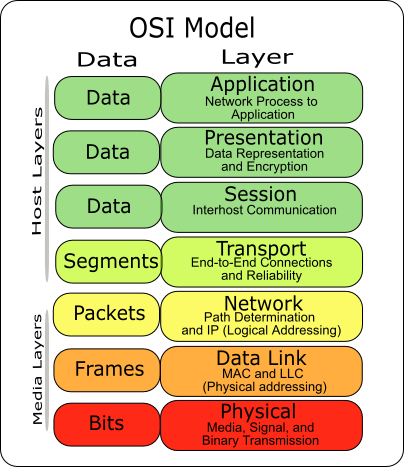
\includegraphics[width=0.4\textwidth,]{fig/Osi-model-jb.png}
}
\caption{OSI model} \label{fig: OSI model}
\end{figure*}

\begin{figure*}
\centering
{
	\includegraphics[width=0.6\textwidth,]{fig/Osi-model.png}
}
\caption{Data Transfer in OSI model} \label{fig: OSI channel}
\end{figure*}

\subsection{Physical Layer}
Physical Layer specification defines the hardware requirements for the devices. 

802.15.4\cite{802154} standard is supported in many recent WSN devices. Its physical layer specification is intended for embedded devices emphasising low energy, low cost and low speed. Bluetooth Low Energy, BLE, is another candidate for WSN with similar features. \cite{802154BLE} provides a performance comparison of 802.15.4 and BLE.

\subsection{Data Link Layer}

\subsection{Network Layer}

\subsection{Transport Layer}

\subsection{Application Layer}

%\cite{802154Sec} discusses some security concerns in 802.15.4.  LLSEC\cite{LLSEC} is the implementation of 802.15.4 security in Contiki.
%
%tinydtls\cite{tinydtls} is the implementation of DTLS we used in DTLS related experiments.
%
%To our knowledge, this is the first work of application fingerprinting through traffic analysis over wireless sensor network.

\section{Security Related Work}

\section{Potential Leakage Sources}